\begin{figure}[t]
\begin{tabular}{cc}
\begin{subfigure}[b]{0.48\textwidth}
{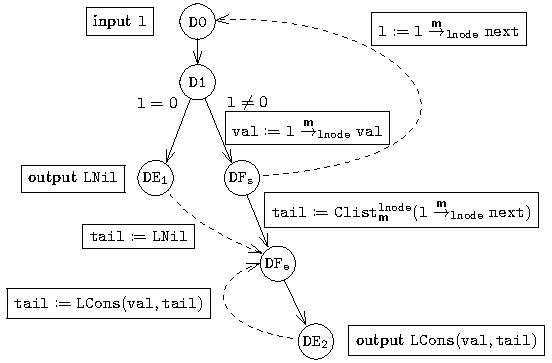
\includegraphics[scale=0.9]{chapters/figures/figClistCfg.pdf}}
\vspace{5px}
\caption{\label{fig:reconsProg}Reconstruction Program}
\end{subfigure}%
&
\begin{subfigure}[b]{0.52\textwidth}
{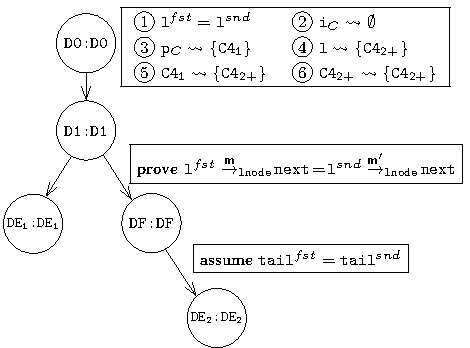
\includegraphics[scale=0.9]{chapters/figures/figClistProductCfg.pdf}}
\vspace{22px}
\caption{\label{fig:reconsPCFG}Recons-PCFG}
\end{subfigure}%
%&
%\begin{subfigure}[b]{0.17\textwidth}
%\includegraphics[scale=0.8]{figMallocPointsToGraph.pdf}
%\caption{\label{xxx}XXX}
%\end{subfigure}%
\\
\end{tabular}
\caption{\label{fig:recons}The reconstruction program for {\tt Clist}$_m^{\tt lnode}({\tt l}_C)$ and recons-PCFG between reconstruction programs of {\tt Clist}$_m^{\tt lnode}({\tt l}_C)$ and {\tt Clist}$_{m'}^{\tt lnode}({\tt l}_C)$. In \cref{fig:reconsProg}, {\tt D0} represents the unrolling procedure entry node, and the square boxes show the transfer functions of the unrolling procedure (\cref{eqn:clist}). The dashed edges represent a recursive function call. In \cref{fig:reconsPCFG}, the square box to the right of node {\tt D0:D0} contains the inferred invariants for this recons-PCFG.}
\end{figure}
